%!TEX root = proj_report_outline.tex
\chapter{Requirements}\label{C:requirements}

\section{Previous Work}

To contextualise the requirements identified this section first introduces Callaghan Innovation's previous work on PitchHub. Callaghan Innovation began work on the idea of PitchHub in 2013. Since this time Callaghan Innovation has discerned what functionality a collaborative innovation platform like PitchHub needs to fulfil it's aim of driving innovation by connecting the roles identified in Section \ref{commonRolesInInnovation}. From this point onward Callaghan Innovation's initial conceptualisation of PitchHub is referred to as as PitchHub alpha.

\subsection{Pitch Cards Conceptualisation}
As discussed in Chapter \ref{background} the innovation community has a very specific purpose and therefore requires special kind of user participation/interaction \cite{Jruby:online}. The interaction which PitchHub facilitates is orientated around ideas. The notion of an idea is very general and ambiguous and to be able to convey it clearly requires precision. To facilitate this PitchHub structures ideas in the form of `Pitch Cards'. Pitch Cards describe ideas in basically the same way CRC cards describe classes, by highlighting the fundamentals and leaving out the non-essential. Callaghan Innovation designed Pitch Cards to explicitly support collaboration between the roles around a Pitch Card. To do this each Pitch Card is made up of a number of Pitch Points which relate to a role. Figure \ref{fig:pitch_card_original} displays PitchHub alpha's Pitch Card concept.
\begin{figure}[ht]
    \centering
    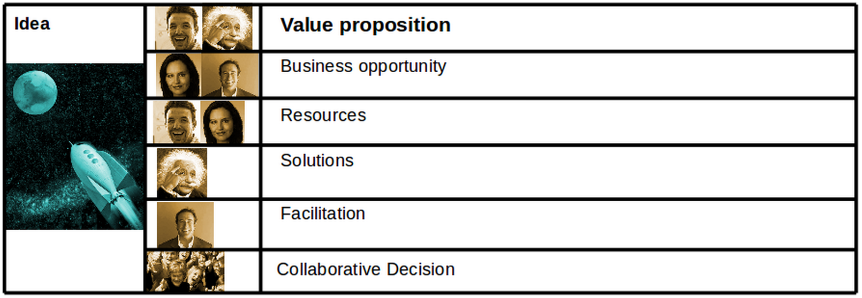
\includegraphics[width=0.8\textwidth]{pitch_card_original}
    \caption{PitchHub alpha's design for a Pitch Card describes an idea with the following Pitch Points: Value Proposition (Any role, describing the idea's value), Business Opportunity (Challenger), Resources (Enabler), Solutions (Solver), Facilitation (Facilitator), Collaborative Decision (Any role, voting on the idea).}
    \label{fig:pitch_card_original}
\end{figure}

\subsection{Collaboration Conceptualisation}
Collaboration on PitchHub is actioned through users making suggestions and comments on these Pitch Points. This is ultimately how PitchHub offers the explicit support of collaboration between roles. Collaboration on PitchHub can be seen as a negotiation, where Pitch Card initiator's describe the idea, and suggestions from the community on the various Pitch Points are then accepted or rejected by the initiator. Accepted suggestions then update the Pitch Point, while rejected Pitch Points just serve as a record of the discussion. Beyond this negotiation of content, collaboration on PitchHub also features negotiation of visibility of content. Figure \ref{fig:pitch_card_original_collaboration} displays an example of PitchHub alpha's PitchCard view.
\begin{figure}[ht]
    \centering
    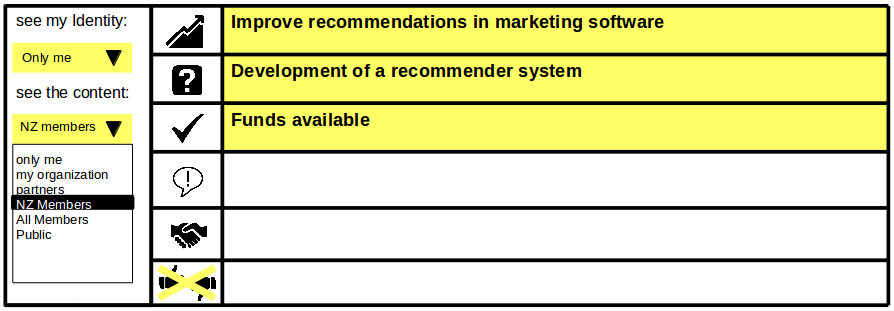
\includegraphics[width=0.8\textwidth]{pitch_card_original_collaboration}
    \caption{PitchHub alpha's design for a Pitch Card's visibility scope as seen from a Pitch Card initiator's view.}
    \label{fig:pitch_card_original_collaboration}
\end{figure}

\section{Methodology}
The software methodology adopted in this project has been an agile, iterative approach. Each iteration is approximately one week in length and consists of the following actions: requirements analysis, requirements validation, design, development, testing, and documentation. During the early stages of the project identifying all of the requirements in a waterfall-like approach was infeasible as this would have required large contiguous amounts of time, of which Callaghan Innovation would not have been able to provide. So in keeping with the agile approach requirements were gathered progressively during client meetings and through the already completed conceptual work. 

\section{Design Requirements}\label{S:designRequirements}
The following functional requirements were identified as being key to the success of the project:

\paragraph{D1: The prototype must enable the innovation community to collaborate.}

The most significant requirement is to ensure that the user stories specified by Callaghan Innovation are fulfilled. The prototype must support these interactions in a sensible manner. Focusing on ideas, rather than people, users should be able to initiate and collaborate on the execution of innovative ideas.

\paragraph{D2.1:  The prototype must enable users to scope the disclosure of their content/identity.}

An interaction behaviour must be developed such that users are able to negotiate the scope of their content to prevent unwanted attention. If users do not wish to disclose their identity or wish to use a scope this behaviour must be supported. This protects users from accidental disclosure.

\paragraph{D2.2: The prototype must provide auditing functionality.}

In order for users to trust that the other users who have viewed their IP are not simply copying it, users must have the ability to audit who has seen their contributions. This enables users to track the movement of their IP and also discourage users from acting unfaithfully.

\paragraph{D2.3: The prototype must store sensitive data securely.}

In order for users to feel safe contributing what may be commercially sensitive information, all data of this nature must be stored in a secure manner. This protects users from malicious disclosure.

\paragraph{D3:  The prototype must be portable and extensible.}

Given the varying degrees of technical skills of the stakeholders at Callaghan Innovation the prototype must be able to be run and extended with minimal effort. The prototype must therefore consider technologies that support ease-of-use over the entire SDLC.

\paragraph{D4: The prototype must be performant.}

In order to facilitate collaboration within the online innovation community the prototype must enable users to fluently use the platform without distraction. It is well-known that extended load/wait times degrade overall user satisfaction and also increase the likelihood of users abandoning operations \cite{SiteSpeed1:online}\cite{TheAverage:online}\cite{HowL7:online}.

\paragraph{D5: The prototype must support a distributed architecture.}

The ability to easily/efficiently scale to meet user demand is a highly desirable property for web systems today. The prototype should use a distributed architecture to achieve this scalability. Consideration must be given as to how redundancy and security operate within the system's distributed context.

